\documentclass[11pt]{article}


\usepackage{epsfig}
\usepackage{graphicx}
\usepackage{latexsym}
\usepackage{amsmath}
\usepackage{amssymb}
\usepackage{tikz}
\usetikzlibrary{arrows}
\usepackage{setspace}
\doublespacing

\setlength{\textwidth}{6.0in}
\setlength{\oddsidemargin}{.1in}
\setlength{\textheight}{21.5cm}
\setlength{\topmargin}{-1.cm}

\setlength{\parindent}{2 ex}
\def\noi{\noindent}
\def\sma{\smallskip}
\def\med{\medskip}
\def\big{\bigskip}

\newtheorem{theorem}{Theorem}
\newtheorem{proposition}{Proposition}
\newtheorem{lemma}{Lemma}
\newtheorem{corollary}{Corollary}
\newtheorem{conjecture}{Conjecture}
\newtheorem{definition}{Definition}
\newtheorem{claim}[theorem]{Claim}
\newtheorem{lem}[theorem]{Lemma}
\newtheorem{prob}{Problem}
\newcommand{\cqfd}{\mbox{}\hfill $\Box$ \medskip}
\newcommand{\comment}[1]{}

\title{Ensemblign}
\date{6 December 2013} %Clears date field from title
\author{William Heaton}
\begin{document}
\maketitle

\paragraph{Introduction\newline}
\par{
Ensemblign is a novel multiple sequence alignment algorithm for estimating the MLE multiple alignment or sampling from the posteriori distribution of multiple alignments. It takes the approach of first computing all pairwise alignments and then combining them into a multiple alignment. But it improves on other algorithms with this approach because it benefits from the posteriori distribution of pairwise alignments generated by the forward/backward algorithm hidden markov model alignment outlined in Durbin and Eddy\cite{Durbin} and then computes the highest probability self consistent multiple alignment via a modified Karger's algorithm. Due to the fact that Karger's algorithm is a monte carlo approximation algorithm, we can also sample from the distribution of posteriori multiple alignments. Armed with this algorithm, biologists can sample not just MLE, but typical explanations of their multiple sequence data. But to be honest, I am not sure how good or fast this will be so I just need to code it up and test on some standard MSA benchmark data to see.

}
%\par{
 %}
 
 
\paragraph{Motivation\newline}
%\par{



%}


\paragraph{Goals\newline}
%\par{

%}

\paragraph{Assumptions}
\par{
Every algorithm has a assumptions. Only the prudent ones list them.
\itemize{
\item We assume that all sequences input have arrisen from the same source molecule with the variations coming from mutation or sequencing error. If this is not the case, then the math and the algorithm will not be correct. 
\item Because dissimilarities due to mutation and sequencing error will conform to different distributions, the scoring of each should be for that partucular case.
\item I will list other assumptions here as they occur to me.

}

}



\paragraph{Pairwise Alignment\newline}
\par{
There exists a considerable literature on pairwise alignments that we need not discuss at length. The first description of the dynamic programming alignment algorithm was by Needleman and Wunsch\cite{NeedlemanWunsch} when was then generalized from global to local alignment by Smith and Waterman.\cite{SmithWaterman}. But the pairwise alignment algorithm used for this project is the HMM formulation first described by <citation needed> and laid out in \cite{Durbin} chapter <look up chapter>. The benefit of this latter method is that not just the single highest scoring alignment is generated, but for every pair of nucleotides that could be aligned between the two sequences, a probability is generated representing the posterior probability over all possible alignments of the two sequences weighted on the likelihood of those alignments. 
}
\par{
First we will consider the case of non-HMM alignment and then we will extend it to the more complicated but more powerful case. These algorithms construct an ordered set of matched pairs of nucleotides (or pair of nucleotide and gap) between the two input sequences such that a score function on the level of error admitted by the alignment is optimized (maximized or minimized depending on scoring metric over all possible alignments).  Since this is all previous work not novel to our method we will simply refer the reader to appropriate sources and provide one example.}

\begin{figure}[h!]
 \caption{Pairwise Alignment.}
\begin{center}
\begin{tikzpicture}[scale=1]

	\tikzstyle alignment lines=[densely dashed, thick];
	\tikzstyle fragment lines=[thick];
	\tikzstyle probe lines=[thick];

		\foreach \x/\label/\char in {0/0/a,1/1/t,2/2/t,3/3/c,4/4/t,5/5/c,6/6/g}
			\node at (\x,1) {\char};
    \foreach \x/\label/\char in {0/0/a,1/1/t,2/2/t,3/3/c,4/4/t,5/5/c,6/6/g}
  		\node at (\x,1.35) {\label};

		\foreach \x/\y/\char in {2/0/t,3/1/c,4/2/t,5/3/c,6/4/g,7/5/g,8/6/c}
			\node at (\x,0) {\char};
    \foreach \x/\y/\char in {2/0/t,3/1/c,4/2/t,5/3/c,6/4/g,7/5/g,8/6/c}
  		\node at (\x,-.35) {\y};
		
		\foreach \x in {2,3,4,5,6}
			\draw[alignment lines, xshift=\x cm] (0,.18) -- (0,.82);

\end{tikzpicture}

\end{center}
\end{figure}
\begin{center}
Giving the ordered set of pairs for this alignment as $\{\{v^0_2,v^1_0\},\{v^0_3,v^1_1\},\{v^0_4,v^1_2\},\{v^0_5,v^1_3\},\{v^0_6,v^1_4\}\}$
\end{center}

The aligned pairs of monomers in such an alignment are likely to represent the same particular locus in the source molecule.

\par{
Later in this document it will become useful to diagram this alignment as a graph where the monomers are vertices and an edge represents the fact that those two monomers have been aligned.  This seems rather trivial for the pairwise case but will become more complex later.  An example of this can be seen in Figure 2.
}
\begin{figure}[h!]
\begin{center}
\begin{tikzpicture}[scale=1]

	\tikzstyle probe=[thick];
	\tikzstyle fragment lines=[thick];
	\tikzstyle probe lines=[thick];

	\foreach \x/\label in {-5.8/0,-5.5/1,-2.75/2,-2.5/3,0/4,2/5,3/6}
			\filldraw[probe,xshift=\label cm] (0,1) circle (1.75pt) node[anchor=south] {$v^0_\label$};
			
			\foreach \x/\label in {2/0,3/1,4/2,5/3,6/4,7/5,8/6}
			\filldraw[probe,xshift=\x cm] (0,0) circle (1.75pt) node[anchor=north] {$v^1_\label$};
			
			\foreach \x in {2,3,4,5,6}
				\draw[probe lines,xshift=\x cm] (0,0) -- (0,1);

\end{tikzpicture}
\caption{Pairwise Alignment: Graph Representation. }

\end{center}
\end{figure}


%\paragraph{Pairwise Alignment Errors\newline}
%\par{
%While representing the optimal scoring alignment, a pairwise alignment can have errors.  Generally speaking, then, we can define two kinds of errors in a pairwise alignment: missing edges and extra edges.  That is to say two monomers that should have been aligned as they represent measurements of the same location in the genome but were not aligned and two monomers that should not have been aligned because they represent two different locations in the genome but were aligned.  The diagrams below demonstrate some causes of alignment errors.  Note that inserted monomers are colored red here.  And the deletions are shown by an outline shaded red in the place where the monomer should have occurred.  In real data when comparing two measurements, we do not know which monomers occured in the source molecule and which monomers are a result of error or mutation so we are displaying this information for demonstration purposes only. The error in the data must be modeled and incorporated in a scoring system that minimizes these alignment errors <citation needed>.
%}


\paragraph{\newline Multiple Alignment\newline}


\par{
We shall describe the homology between a set of sequences with a multiple alignment.  The purpose of a multiple alignment is to match input nucleotides in sets that reflect the nucleotide occurrences on the source molecule from which the inputs originated.  In structure, a multiple alignment is an ordered set of sets of nucleotides. Each set (\textbf{aligned point}) consists of at most one monomer on each measurement.  Additionally, each monomer on each sequence is present in at most one set. Finally, the sets must obey the ordering principle: if monomers a, b, and c occur on the same input sequence such that b lies after a and before c, and each of a, b, and c is in an aligned set, the the aligned set containing b lies after the aligned set which contains a and before that which contains c in the multiple alignment.  Intuitively, each aligned point consists of those monomers that "match," i.e. that are measurements of the same locus in the source molecule.
}

\begin{figure}[h!]

\begin{center}
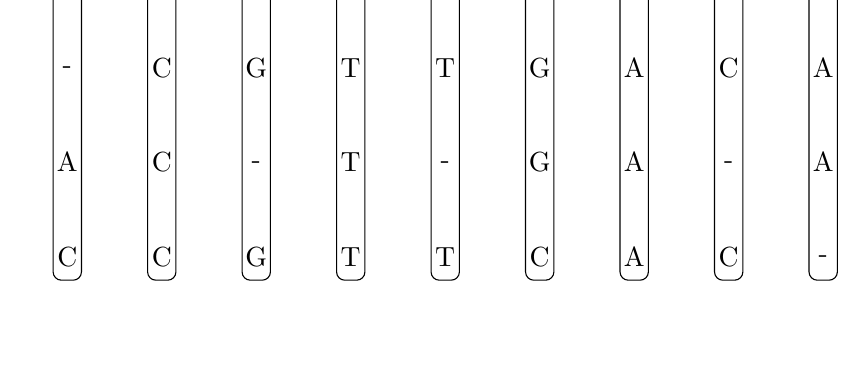
\begin{tikzpicture}[scale=1.2]

	\tikzstyle alignment lines=[densely dashed, thick];
	\tikzstyle fragment lines=[thick];
	\tikzstyle probe lines=[thick];
	\tikzstyle multiple alignment=[rounded corners=3pt];

	%\draw[fragment lines] (-6,5) node[anchor=east] {$v^0$} -- (3.5,5);
		\foreach \x/\y in {0/A,1/C,2/G,3/-,4/-,5/G,6/A,7/G,8/A}
			\node at (\x,5) {\y};
      %\draw[probe lines,xshift=\x cm] (0,4.85) -- (0,5.15) node[anchor=south] {$\label$};

	%\draw[fragment lines] (-5.5,4) node[anchor=east] {$v^1$}  -- (4,4);
		  	\foreach \x/\y in {0/-,1/C,2/G,3/T,4/T,5/G,6/A,7/C,8/A}
			  \node at (\x,4) {\y};
      %\draw[probe lines,xshift=\x cm] (0,4.15) node[anchor=south] {$\y$} -- (0,3.85) ;
			
		%	\draw[fragment lines] (-4.5,3) node[anchor=east] {$v^2$}  -- (4.5,3);
	  	\foreach \x/\y in {0/A,1/C,2/-,3/T,4/-,5/G,6/A,7/-,8/A}
			\node at (\x,3) {\y};
      %\draw[probe lines,xshift=\x cm] (0,3.15)node[anchor=south] {$\y$} -- (0,2.85) ;
			
		%			\draw[fragment lines] (-4,2) node[anchor=east] {$v^3$}  -- (5,2);
	  	\foreach \x/\y in {0/C,1/C,2/G,3/T,4/T,5/C,6/A,7/C,8/-}
			\node at (\x,2) {\y};
      %\draw[probe lines,xshift=\x cm] (0,2.15) node[anchor=south] {$\y$} -- (0,1.85) ;
			
		%						\draw[fragment lines] (-3.5,1) node[anchor=east] {$v^4$}  -- (5.5,1);
		%\foreach \x/\y in {/0,-2.5/1,0/2,2/3,3/4,4.5/5,5/6}
		%	\draw[probe lines,xshift=\x cm] (0,1.15) node[anchor=south] {$\y$} -- (0,.85) ;
			
		%						\draw[fragment lines] (-3,0) node[anchor=east] {$v^5$}  -- (6,0);
		%\foreach \x/\y in {-2.75/0,-2.5/1,0/2,2/3,3/4,4.5/5,5/6}
	%		\draw[probe lines,xshift=\x cm] (0,.15) node[anchor=south] {$\y$} -- (0,-.15) ;
		
		\draw[multiple alignment] (-.15,1.75) rectangle (.15,5.25);
		\draw[multiple alignment] (.85,1.75) rectangle (1.15,5.25);
		\draw[multiple alignment] (1.85,1.75) rectangle (2.15,5.25);
		\draw[multiple alignment] (2.85,1.75) rectangle (3.15,5.25);
		\draw[multiple alignment] (3.85,1.75) rectangle (4.15,5.25);
      	\draw[multiple alignment] (4.85,1.75) rectangle (5.15,5.25);
          	\draw[multiple alignment] (5.85,1.75) rectangle (6.15,5.25);
              	\draw[multiple alignment] (6.85,1.75) rectangle (7.15,5.25);
                  	\draw[multiple alignment] (7.85,1.75) rectangle (8.15,5.25);

\end{tikzpicture}
 \caption{Multiple Alignment}
\end{center}
\end{figure}

\paragraph{Graph Conception of a Multiple Alignment\newline}
\par{
Recall the graph representation of pairwise alignments from figure 2.  We will now extend this to a multiple alignment.  The aligned points that make up a multiple alignment are equivalence classes, such that every pair of monomers in such a set has the relation ``are homologous." A \textbf{graph} can built representing these pairwise relations, wherein a vertex $v^{i}_j$ represents the $j^{th}$ monomer on sequence $i$ and the (undirected) edge ($v^{i}_j$,$v^k_l$) represents that $v^i_j$ and $v^k_l$ are homologous with respect to the sequence of common origin.  By way of notation, $v^i_j.m = i$ and $v^i_j.e = j$.  Because, by definition, those monomers in a given aligned point are homologous to one another and to no other monomers, each connected component in this graph is fully connected and consists of the monomers in one aligned point.\cite{Corel}
}

\begin{figure}[h!]
\begin{center}
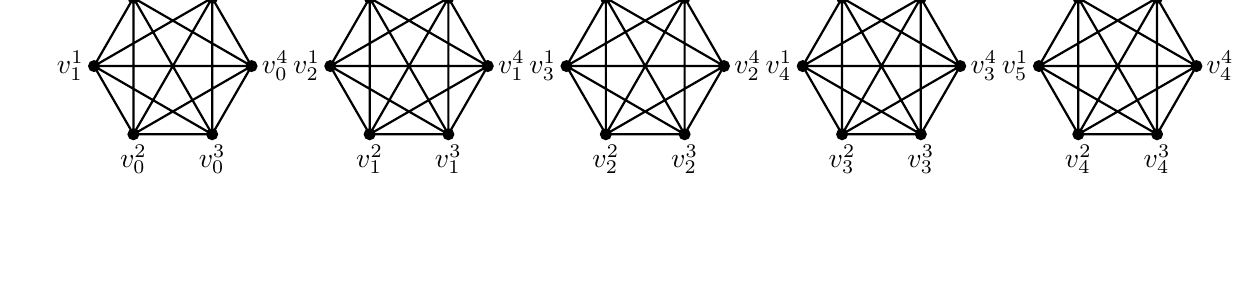
\begin{tikzpicture}[scale=1]

	\tikzstyle probe=[thick];
	\tikzstyle fragment lines=[thick];
	\tikzstyle probe lines=[thick];

	
	\filldraw[probe] (.5,1.732) circle (1.75pt) node[anchor=south] {$v^0_2$};
	\filldraw[probe] (0,.866) circle (1.75pt) node[anchor=east]{$v^1_1$};
	\filldraw[probe] (1.5,1.732) circle (1.75pt) node[anchor=south] {$v^5_0$};
	\filldraw[probe] (2,.866) circle (1.75pt) node[anchor=west]{$v^4_0$};
	\filldraw[probe] (.5,0) circle  (1.75pt) node[anchor=north]{$v^2_0$};
	\filldraw[probe] (1.5,0) circle  (1.75pt) node[anchor=north]{$v^3_0$};
	\draw[probe lines] (.5,1.732) -- (0,.866) -- (1.5,1.732) -- (2,.866) -- (.5,0) -- (1.5,1.732) -- (1.5,0) -- (.5,1.732) -- (1.5,1.732) -- (2,.866) -- (.5,1.732) -- (.5,0) -- (1.5,0) --  (2,.866) -- (.5,0) -- (.5,1.732) -- (2,.866) -- (0,.866) -- (.5,0) -- (1.5,0)--(0,.866);
	
	
		\filldraw[probe] (3.5,1.732) circle (1.75pt) node[anchor=south] {$v^0_3$};
	\filldraw[probe] (3,.866) circle (1.75pt) node[anchor=east]{$v^1_2$};
	\filldraw[probe] (4.5,1.732) circle (1.75pt) node[anchor=south] {$v^5_1$};
	\filldraw[probe] (5,.866) circle (1.75pt) node[anchor=west]{$v^4_1$};
	\filldraw[probe] (3.5,0) circle  (1.75pt) node[anchor=north]{$v^2_1$};
	\filldraw[probe] (4.5,0) circle  (1.75pt) node[anchor=north]{$v^3_1$};
	\draw[probe lines] (3.5,1.732) -- (3,.866) -- (4.5,1.732) -- (5,.866) -- (3.5,0) -- (4.5,1.732) -- (4.5,0) -- (3.5,1.732) -- (4.5,1.732) -- (5,.866) -- (3.5,1.732) -- (3.5,0) -- (4.5,0) --  (5,.866) -- (3.5,0) -- (3.5,1.732) -- (5,.866) -- (3,.866) -- (3.5,0) -- (4.5,0)--(3,.866);
	
		\filldraw[probe] (6.5,1.732) circle (1.75pt) node[anchor=south] {$v^0_4$};
	\filldraw[probe] (6,.866) circle (1.75pt) node[anchor=east]{$v^1_3$};
	\filldraw[probe] (7.5,1.732) circle (1.75pt) node[anchor=south] {$v^5_2$};
	\filldraw[probe] (8,.866) circle (1.75pt) node[anchor=west]{$v^4_2$};
	\filldraw[probe] (6.5,0) circle  (1.75pt) node[anchor=north]{$v^2_2$};
	\filldraw[probe] (7.5,0) circle  (1.75pt) node[anchor=north]{$v^3_2$};
	\draw[probe lines] (6.5,1.732) -- (6,.866) -- (7.5,1.732) -- (8,.866) -- (6.5,0) -- (7.5,1.732) -- (7.5,0) -- (6.5,1.732) -- (7.5,1.732) -- (8,.866) -- (6.5,1.732) -- (6.5,0) -- (7.5,0) --  (8,.866) -- (6.5,0) -- (6.5,1.732) -- (8,.866) -- (6,.866) -- (6.5,0) -- (7.5,0)--(6,.866);
	
		\filldraw[probe] (9.5,1.732) circle (1.75pt) node[anchor=south] {$v^0_5$};
	\filldraw[probe] (9,.866) circle (1.75pt) node[anchor=east]{$v^1_4$};
	\filldraw[probe] (10.5,1.732) circle (1.75pt) node[anchor=south] {$v^5_3$};
	\filldraw[probe] (11,.866) circle (1.75pt) node[anchor=west]{$v^4_3$};
	\filldraw[probe] (9.5,0) circle  (1.75pt) node[anchor=north]{$v^2_3$};
	\filldraw[probe] (10.5,0) circle  (1.75pt) node[anchor=north]{$v^3_3$};
	\draw[probe lines] (9.5,1.732) -- (9,.866) -- (10.5,1.732) -- (11,.866) -- (9.5,0) -- (10.5,1.732) -- (10.5,0) -- (9.5,1.732) -- (10.5,1.732) -- (11,.866) -- (9.5,1.732) -- (9.5,0) -- (10.5,0) --  (11,.866) -- (9.5,0) -- (9.5,1.732) -- (11,.866) -- (9,.866) -- (9.5,0) -- (10.5,0)--(9,.866);
	
		\filldraw[probe] (12.5,1.732) circle (1.75pt) node[anchor=south] {$v^0_6$};
	\filldraw[probe] (12,.866) circle (1.75pt) node[anchor=east]{$v^1_5$};
	\filldraw[probe] (13.5,1.732) circle (1.75pt) node[anchor=south] {$v^5_4$};
	\filldraw[probe] (14,.866) circle (1.75pt) node[anchor=west]{$v^4_4$};
	\filldraw[probe] (12.5,0) circle  (1.75pt) node[anchor=north]{$v^2_4$};
	\filldraw[probe] (13.5,0) circle  (1.75pt) node[anchor=north]{$v^3_4$};
	\draw[probe lines] (12.5,1.732) -- (12,.866) -- (13.5,1.732) -- (14,.866) -- (12.5,0) -- (13.5,1.732) -- (13.5,0) -- (12.5,1.732) -- (13.5,1.732) -- (14,.866) -- (12.5,1.732) -- (12.5,0) -- (13.5,0) --  (14,.866) -- (12.5,0) -- (12.5,1.732) -- (14,.866) -- (12,.866) -- (12.5,0) -- (13.5,0)--(12,.866);

\end{tikzpicture}
\caption{Multiple Alignment: Graph Representation. As you can see this results in a series of clique subgraphs.}

\end{center}
\end{figure}

\paragraph{Multiple Alignment as the Union of Pairwise Alignments\newline}
\par{
Let us call this multiple alignment graph $G$, consisting of a set of vertices $V$ and a set of edges $E$. We can, for each pair $j$ and $l$, define $E_{jl}=E_{lj}=(u,v)$ in E such that $u.m = j$ and $v.m = l$. Since each pair of monomers $(u,v)$ in E comes from exactly one pair of different sequences, the set of all $E_{jl}$ is a partitioning of $E$. $E_{jl}$ defines a \textbf{pairwise} alignment between sequences $j$ and $l$, consisting of the pairs of homologous monomers between these two sequences.  That {$E_{jl}$} is a partitioning of $E$ is also to say that $E$ is the union over all such pairwise alignments.  So one way to determine the perfect multiple alignment between a collection of sequences is to take the union of perfect pairwise alignments.
}
\par{
But as a result of sequencing error or mutation, a given pairwise alignment is rarely perfect.   Consider two sequences, x and y, with monomers $x_{1...m}$ and $y_{1...n}$.   Each monomer derives either from a source molecule site $\gamma$ or from an insertion.  In the latter case, the monomer is not homologous to a monomer on any other sequence and a perfect pairwise alignment will not include this monomer in a matched pair.  In the former case, this monomer will be matched if and only if the other sequence has an monomer deriving from $\gamma$.  So the ordered set of aligned points in a perfect pairwise alignment consists of one matched pair for each monomer in the intersection of true monomers in the two sequences.
}

\begin{figure}[h!]
\begin{center}
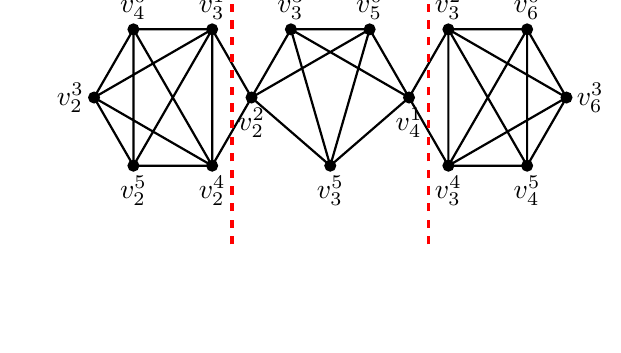
\begin{tikzpicture}[scale=1]

	\tikzstyle probe=[thick];
	\tikzstyle fragment lines=[thick];
	\tikzstyle probe lines=[thick];

	
	\filldraw[probe] (.5,1.732) circle (1.75pt) node[anchor=south] {$v^0_4$};
	\filldraw[probe] (0,.866) circle (1.75pt) node[anchor=east]{$v^3_2$};
	\filldraw[probe] (1.5,1.732) circle (1.75pt) node[anchor=south] {$v^1_3$};
	\filldraw[probe] (2,.866) circle (1.75pt) node[anchor=north]{$v^2_2$};
	\filldraw[probe] (.5,0) circle  (1.75pt) node[anchor=north]{$v^5_2$};
	\filldraw[probe] (1.5,0) circle  (1.75pt) node[anchor=north]{$v^4_2$};
	\draw[probe lines] (.5,1.732) -- (0,.866) -- (1.5,1.732)  -- (1.5,1.732) -- (1.5,0) -- (.5,1.732) -- (1.5,1.732) -- (.5,1.732) -- (.5,0) --(0,.866) --(1.5,0) --(.5,0) --(1.5,1.732) -- (1.5,0) -- (2,.866);
	
	
  \filldraw[probe] (2.5,1.732) circle (1.75pt) node[anchor=south] {$v^3_3$};
	\filldraw[probe] (3.5,1.732) circle (1.75pt) node[anchor=south] {$v^0_5$};
	\filldraw[probe] (3,0) circle  (1.75pt) node[anchor=north]{$v^5_3$};
	\draw[probe lines] (1.5,1.732) -- (2,.866) -- (3.5,1.732) -- (4,.866) -- (3,0) -- (3.5,1.732) -- (3,0) -- (2.5,1.732) -- (3.5,1.732) -- (4,.866) -- (2.5,1.732) -- (3,0) --  (4,.866) -- (3,0) -- (2.5,1.732)  -- (2,.866) -- (3,0);
	
		\filldraw[probe] (4.5,1.732) circle (1.75pt) node[anchor=south] {$v^2_3$};
	\filldraw[probe] (4,.866) circle (1.75pt) node[anchor=north]{$v^1_4$};
	\filldraw[probe] (5.5,1.732) circle (1.75pt) node[anchor=south] {$v^0_6$};
	\filldraw[probe] (6,.866) circle (1.75pt) node[anchor=west]{$v^3_6$};
	\filldraw[probe] (4.5,0) circle  (1.75pt) node[anchor=north]{$v^4_3$};
	\filldraw[probe] (5.5,0) circle  (1.75pt) node[anchor=north]{$v^5_4$};
	\draw[probe lines] (4.5,1.732)  -- (5.5,1.732) -- (6,.866) -- (4.5,0) -- (5.5,1.732) -- (5.5,0) -- (4.5,1.732) -- (5.5,1.732) -- (6,.866) -- (4.5,1.732) -- (4.5,0) -- (5.5,0) --  (6,.866) -- (4.5,0) -- (4.5,1.732) -- (6,.866)  -- (4.5,0) -- (5.5,0) -- (4.5,0) -- (4,.866) -- (4.5,1.732);
	
	
	\draw[red,dashed, very thick] (4.25,-1) -- (4.25,2.732);
	
	\draw[red,dashed, very thick] (1.75,-1) -- (1.75,2.732);
	

\end{tikzpicture}
\caption{Multiple Alignment: Graph Representation. This alignment graph contains multiple \textbf{contradictions}.  Note that the vertices have been rearranged spatially for ease of viewing the graph.  The broken red lines indicate the edges that must be cut in order to obtain the contradiction-free multiple alignment that best explains all of the pairwise alignments.}
\end{center}
\end{figure}


\paragraph{Modified-Karger's Algorithm for Contradiction Separation\newline}
\par{
Suppose that we have performed pairwise alignments between all pairs of input sequences.  Consider the set of edges $E^\prime$ (and the graph $G^\prime={V,E^\prime}$) formed by taking the union of these imperfect pairwise alignments.  $E^\prime$ differs from the perfect solution $E$ in its missing and extra edges.  Most importantly, the extra edges mean that $E^\prime$ has edges between what would be separated components in $E$.  (Additionally, some edges are missing within what would be connected components in $E$. These missing edges are less of a concern under the assumption that we have at least several sequences because it is very unlikely that enough edges might be missing to separate a connected component into two or more components.) In order to recover $E$ as best possible, we set about removing the extra edges from $E^\prime$.
}
\par{
The extra edges in $E^\prime$ have the property that they introduce \textbf{contradictions}.  Let us define a contradiction as a connected component in $G^\prime$ that contains two or more different vertices from the same sequence.  This means that the multiple alignment implicit from $G^\prime$ currently counts two monomers on one sequence as arising from a single monomer in the underlying true sequence of the source molecule.  This is always an error because each aligned point in our multiple alignment should correspond to a particular monomer $\gamma$ in the sequence of common origin and it is impossible for two sites on the same sequence to be homologous to the same $\gamma$.  One important step towards fixing $E^\prime$ is to separate these \textbf{contradictory components} into non-contradictory ones.
<add figure detailing an example of contradictory pairwise alignments>}




\par{
Under the presumption that most edges in $E^\prime$ are correct, a natural way to fix these contradictions is to find a min-cut such that no contradictions remain.  We use a novel, modified version of Karger's Algorithm to find this min-cut.  Karger's Algorithm is a probabilistic algorithm that finds the min-cut of a graph by finding strongly connected components and then severing them from one another.  These strongly connected components are discovered by "contracting" edges at random until only two nodes remain.  To contract an edge is to remove the edge and combine its end nodes into one node retaining all other edges therefore allowing multiple edges between two nodes.  The selected cut itself is the set of all edges remaining when no further contraction is allowed.  This process can of course fail to find the min-cut.  Consider for instance that the first edge contracted at random happens to be an edge that is in the min cut.  For this reason we must perform this succession of contractions many times in parallel and selecting the minimum cut among these iterations, the algorithm offers high probability of finding the min-cut.  Because strongly connected components contain far more edges than other areas of the graph, these areas get contracted earlier with higher probability.  This convenient property of highly connected components allows for very high probability of finding the real min-cut with surprisingly few iterations.  This run time can be further improved by a modification known as the Karger-Stein algorithm.  In our case, we impose the additional constraint that no two vertices representing monomers on the same sequence can be contracted.  This constraint is natural because the fully-contracted vertices at the end of Karger's Algorithm are identical to the \textbf{aligned points} our multiple alignment seeks to recover.  As such, our modified Karger's Algorithm contracts edges at random without violating constraints until no contractions are allowed under the constraints.  The min-cut selected by this modified Karger's Algorithm represents a likely selection of the extra edges in $E^\prime$ and, in any case, results in an ordered set of non-contradictory connected components that best explain the set of pairwise alignments.\cite{Karger1}\cite{Karger2}
 As a simplified example, take the following set of fragments.}



\begin{figure}[h!]
\begin{center}
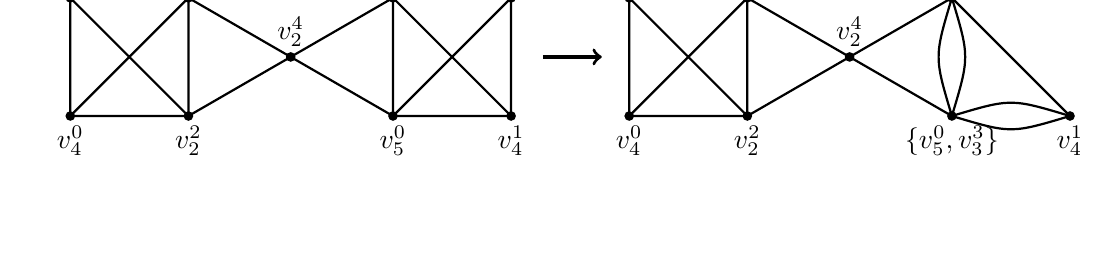
\begin{tikzpicture}[scale=.75]

	\tikzstyle probe=[thick];
	\tikzstyle fragment lines=[thick];
	\tikzstyle probe lines=[thick];

	
	\filldraw[probe] (0,0) circle (1.75pt) node[anchor=north] {$v^0_4$};
	\filldraw[probe] (0,2) circle (1.75pt) node[anchor=south]{$v^1_3$};
	\filldraw[probe] (2,0) circle (1.75pt) node[anchor=north] {$v^2_2$};
	\filldraw[probe] (2,2) circle (1.75pt) node[anchor=south]{$v^3_2$};
  
	\draw[probe lines] (0,0) -- (0,2) -- (2,0) -- (2,2) -- (0,2) -- (2,0) -- (0,0) -- (2,2);
  
	\filldraw[probe] (3.732,1) circle (1.75pt) node[anchor=south] {$v^4_2$};
  
	\draw[probe lines] (3.732,1) -- (5.464,0);
	\draw[probe lines] (3.732,1) -- (5.464,2);
	\draw[probe lines] (3.732,1) -- (2,0);
	\draw[probe lines] (3.732,1) -- (2,2);
	
	\filldraw[probe] (5.464,0) circle (1.75pt) node[anchor=north] {$v^0_5$};
	\filldraw[probe] (7.464,0) circle (1.75pt) node[anchor=north]{$v^1_4$};
	\filldraw[probe] (5.464,2) circle (1.75pt) node[anchor=south] {$v^2_3$};
	\filldraw[probe] (7.464,2) circle (1.75pt) node[anchor=south]{$v^3_3$};
  
	\draw[probe lines] (5.464,0) -- (5.464,2) -- (7.464, 2) -- (5.464,2) -- (7.464,0) -- (5.464,0) -- (7.464,2) -- (7.464,0);
	
	\draw[very thick,->] (8,1) -- (9,1);
	
	\filldraw[probe] (9.464,0) circle (1.75pt) node[anchor=north] {$v^0_4$};
	\filldraw[probe] (9.464,2) circle (1.75pt) node[anchor=south]{$v^1_3$};
	\filldraw[probe] (11.464,0) circle (1.75pt) node[anchor=north] {$v^2_2$};
	\filldraw[probe] (11.464,2) circle (1.75pt) node[anchor=south]{$v^3_2$};
  
	\draw[probe lines] (9.464,0) -- (9.464,2) -- (11.464,0) -- (11.464,2) -- (9.464,2) -- (11.464,0) -- (9.464,0) -- (11.464,2);
	
		\filldraw[probe] (13.196,1) circle (1.75pt) node[anchor=south] {$v^4_2$};
    
	\draw[probe lines] (13.196,1) -- (11.464,0);
	\draw[probe lines] (13.196,1) -- (11.464,2);
	\draw[probe lines] (13.196,1) -- (14.928,0);
	\draw[probe lines] (13.196,1) -- (14.928,2);
	
		\filldraw[probe] (14.928,0) circle (1.75pt) node[anchor=north] {$\{v^0_5,v^3_3\}$};
	\filldraw[probe] (16.928,0) circle (1.75pt) node[anchor=north]{$v^1_4$};
	\filldraw[probe] (14.928,2) circle (1.75pt) node[anchor=south] {$v^2_3$};
  
	\draw[probe lines]  (14.928,2) -- (16.928,0);
	\draw[probe lines] (14.928,0) ..  controls (15.228,1) .. (14.928,2);
	\draw[probe lines] (14.928,0) ..  controls (14.628,1) .. (14.928,2);
	
	\draw[probe lines] (14.928,0) ..  controls (15.928,.3)  .. (16.928,0);
	\draw[probe lines] (14.928,0) ..  controls (15.928,-.3) .. (16.928,0);
		
	

\end{tikzpicture}
\caption{Contraction on edge from $v^0_5$ to $v^3_3$. Edges are drawn at random and contracted if they do not have labels of the same fragment (the superscript here). This process continues until either there are 2 nodes left in the graph and the remaining edges are the ``cut" or no more edges can be contracted given our constraint. This process is then repeated several times and the cut with the fewest cut edges is selected as the most likely.}

\end{center}
\end{figure}


\par{
Karger's Algorithm, along with our modifications, is uniquely suited to this problem.  No other formulation of the min-cut problem (network flow, etc.) can be so simply extended with our constraints.  The operation of Karger's Algorithm consists of a probabilistic sampling of the space of graph cuts.  By introducing our constraints, we simple decline to sample the portion of the space that contains contradictions.  And, if this was not clear, in the simple case in which $E^\prime$ contains no contradictions to begin with we do nothing and just take it as the multiple alignment.  
}


\paragraph{Conclusions\newline}

\par{

}

%\paragraph{Combination Sequencing\newline}
%\par{
%Here I will talk about combination sequencing\cite{Antoniotti}\cite{Zhousingle-molecule}
%}


\bibliographystyle{amsplain}
\bibliography{Ensemblign}
\end{document}